\documentclass{article}

% Matemática
\usepackage{amsmath}    % símbolos matemáticos
\usepackage{amsthm}     % teoremas
\usepackage{amsfonts}   % \mathbb
\usepackage{amssymb}    % \therefore
\usepackage{bm}         % bold math (https://ctan.org/pkg/bm)
\usepackage{abraces}    % \aoverbrace http://ctan.org/pkg/abraces
% https://tex.stackexchange.com/questions/132526/overbrace-and-underbrace-with-square-bracket

\usepackage[makeroom]{cancel}   % \cancel

% Figuras
\usepackage{tikz}                   % gráficos
\usepackage{float}                  % [H]
\usepackage{xcolor}                 % colores https://es.overleaf.com/learn/latex/Using_colours_in_LaTeX

% Formateo
\usepackage{framed}     % env leftbar

% Texto
\usepackage[shortlabels]{enumitem}  % enumerate con letras

% Referencias
\usepackage[colorlinks=true]{hyperref}

% Código
\usepackage{listings}

% Diagramas
\usepackage{tikz}
\usetikzlibrary{automata, arrows, positioning}

\tikzset{
    ->, % makes the edges directed
    >=stealth', % makes the arrow heads bold
    node distance=3cm, % specifies the minimum distance between two nodes. Change if necessary.
    every state/.style={thick}, % sets the properties for each 'state' node
    initial text=$ $, % sets the text that appears on the start arrow
}


\usepackage{mathtools}
% Macros para símbolos
\DeclarePairedDelimiter\ceil{\lceil}{\rceil}
\DeclarePairedDelimiter\floor{\lfloor}{\rfloor}

\newcommand{\BigO}{\mathcal{O}}

% Teoremas, corolarios, etc.
% https://www.overleaf.com/learn/latex/theorems_and_proofs
\theoremstyle{definition} % Para que no salga en italicas

\newtheorem{theorem}{Teorema}
\newtheorem*{theorem*}{Teorema}

\newtheorem{lemma}{Lema}
\newtheorem*{lemma*}{Lema}

\newtheorem{proposition}{Prop.}
\newtheorem*{proposition*}{Prop}

\newtheorem{corollary}{Corolario}
\newtheorem*{corollary*}{Corolario}

\newtheorem{definition}{Def.}
\newtheorem*{definition*}{Def}

\newtheorem*{observation*}{Obs}

% Comandos de AAA
\newcommand{\select}{\upharpoonright}

% Entornos
\newenvironment{nota}[1]
    {\begin{leftbar}\textbf{#1}}
    {\end{leftbar}}

\author{Manuel Panichelli}
\title{Algoritmos, Azar y Autómatas\\Resolución Ejercicios 7 y 8 (selección)}

\begin{document}
\maketitle

\section*{Resultados previos}

\begin{definition}[Selección por prefijos]\label{def:prefix-selection}
    Sea $x = a_1 a_2 \dots$ una palabra infinita sobre el alfabeto $A$, y $L
    \subseteq A^*$ un conjunto de palabras finitas sobre ese alfabeto. Una
    \textbf{selección por prefijo} de $x$ por $L$ es

    $$x \select L = a_{i_1} a_{i_2} a_{i_3} \dots,$$

    donde $i_1, i_2, i_3$ es una enumeración en orden creciente de todos los
    enteros $i$ tales que $a_1 a_2 \dots a_{i - 1} \in L$.

    Ejemplos:

    $x = 01001000100001000001000000100000001\dots$
    \begin{itemize}
        \item $L = (0^* 1)^*$

        $x \select L = 000000000\dots$.

        \item $\bar{L} = (A^* \setminus L) = (0^* 1^*)^* 0$
        
        $x \select \bar{L} = 101010010001\dots$
    \end{itemize}
\end{definition}

\begin{theorem}[Agafonov 1968]\label{teo:norm-select-regular}
    Sea $x \in A^\omega$ normal, y $L \subset A^*$ regular. Luego $x \select L$
    es normal.
\end{theorem}

\begin{proposition}[A la Champernowne]\label{prop:a-la-champ}
    La secuencia de la concatenación de todas las posibles palabras de longitud
    $1, 2, 3, \dots$ en orden lexicográfico para el alfabeto $\{0, 1\}$,

    \[
        01\ \
        00\ 01\ 10\ 11\ \
        000\ 001\ 010\ 011\ 100\ 101\ 110\ 111\ \
        0000\dots
    \]

    es normal.
\end{proposition}

\section*{Ejercicio 7}

Dada una secuencia $a_1 a_2 \dots$ donde los $a_i$ son símbolos del alfabeto,
$pares(x)$ es la subsecuencia de $x$ que se obtiene de tomar los símbolos en las
posiciones pares de $x$. Es decir,

\[
    pares(x) = a_2 a_4 a_6 \dots
\]

Demostrar que si $x$ es una secuencia normal, entonces la subsecuencia
$pares(x)$ es normal.

\begin{proof}
    Usando el Teorema \ref{teo:norm-select-regular}, nos basta con encontrar un
    lenguaje regular $L$ tal que $x \select L = pares(x)$ para probar que
    $pares(x)$ es regular.

    Interpretando la definición de \nameref{def:prefix-selection}, el resultado
    de $x \select L$ es la concatenación de los símbolos de las posiciones
    $i$-ésimas tales que el prefijo de longitud $i - 1$ pertenece al lenguaje
    $L$.

    Por lo tanto, para que $x \select L = pares(x) = a_2 a_4 a_6 \dots$, tienen
    que pertenecer a $L$ los prefijos $a_1,\ a_1 a_2 a_3,\ a_1 a_2 a_3 a_4 a_5$,
    y así. Es decir, los de longitud impar. Entonces nos alcanza con dar un
    lenguaje regular para las cadenas del alfabeto $A$ de longitud impar. El
    lenguaje es el aceptado por el autómata finito $M$, $L = \mathcal{L}(M)$.
    Suponiendo que $A = \{ a_1, \dots a_n \}$,

    \begin{figure}[H]
        \centering
        % M = <Q, sigma, delta, q_0, F>
        \(
            M = \langle
                \{ q_P, q_I \},
                A,
                \delta,
                q_P,
                \{ q_I \}
            \rangle
        \), donde $\delta$ está dada por:

        \vspace{0.5cm}

        % https://www3.nd.edu/~kogge/courses/cse30151-fa17/Public/other/tikz_tutorial.pdf
        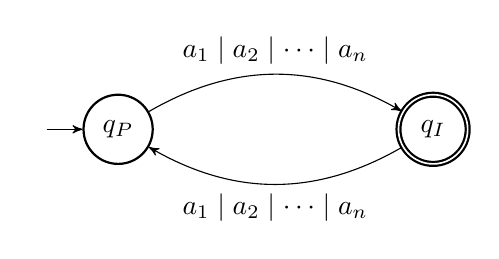
\begin{tikzpicture}
            \node[state, initial] (qp) {$q_P$};
            \node[state, accepting] at (4,0) (qi) {$q_I$};

            \draw
                (qp) edge[bend left, above] 
                    node{$a_1 \mid a_2 \mid \dots \mid a_n$} (qi)
                (qi) edge[bend left, below]
                    node{$a_1 \mid a_2 \mid \dots \mid a_n$} (qp);
        \end{tikzpicture}
    \end{figure}

    Como encontré un autómata que reconoce el lenguaje $L$, $L$ es regular. Y
    como $x \select L = pares(x)$, por el Teorema \ref{teo:norm-select-regular},
    si $x$ es normal, entonces $pares(x)$ también.

\end{proof}

\newpage

\section*{Ejercicio 8}

\textbf{Indicar una forma de selección de subsecuencias tal que no siempre
preserva normalidad. Dar un ejemplo de una secuencia normal donde no se
preserve.}

Para ello, mi estrategia será tomar la cadena normal de la Prop
\ref{prop:a-la-champ},

\begin{align*}
    x =\ &01\\
    &00\ 01\ 10\ 11\\
    &000\ 001\ 010\ 011\ 100\ 101\ 110\ 111\ \\
    &0000\
    0001\
    0010\
    0011\
    0100\
    0101\
    0110\
    0111\
    1000\
    1001\
    1010\
    1011\
    1100\
    1101\
    1110\
    1111\
    \dots
\end{align*}

y mostrar que puedo dar un lenguaje $L$ tal que $x \select L$ no sea normal. Voy
a llamar \textit{bloque} a la concatenación de todas las cadenas de cierta
longitud, por ej. 01 es el bloque de long 1 y $00 01 10 11$ el de long 2. La
idea de $L$ entonces es que contenga los prefijos de las concatenaciones
\textbf{completas} de todos los bloques que forman $x$, y de esa forma va a
pertenecer el primer símbolo del siguiente bloque, que es siempre 0.

El lenguaje $L$ será el aceptado por la máquina de Turing $M$ expresada mediante
un programa (en particular en Python). La función que lo computa es
\texttt{recognize},

\definecolor{codegreen}{rgb}{0,0.6,0}
\definecolor{codegray}{rgb}{0.5,0.5,0.5}
\definecolor{codepurple}{rgb}{0.58,0,0.82}
\definecolor{backcolour}{rgb}{0.95,0.95,0.92}

\lstdefinestyle{mystyle}{
    backgroundcolor=\color{backcolour},   
    commentstyle=\color{codegreen},
    keywordstyle=\color{blue},
    numberstyle=\tiny\color{codegray},
    stringstyle=\color{codepurple},
    basicstyle=\ttfamily\footnotesize,
    breakatwhitespace=false,         
    breaklines=true,                 
    captionpos=b,                    
    keepspaces=true,                 
    numbers=left,                    
    numbersep=5pt,                  
    showspaces=false,                
    showstringspaces=false,
    showtabs=false,                  
    tabsize=2
}

\lstset{style=mystyle}

\begin{lstlisting}[language=Python, caption=Programa que reconoce las cadenas de $L$]
def recognize(word: str) -> bool:
    """
    Reconoce una cadena solo si es un prefijo que coincide con
    un fin de un "bloque" de una cadena "a la Champernowne".
    """

    n = 0
    current_champ = ""
    while len(current_champ) <= len(word):
        if word == current_champ:
            return True
        
        n += 1
        current_champ = champ_up_to(n)
    
    return False

def champ_up_to(n: int) -> str:
    """
    Genera la secuencia "a la Champernowne" hasta el bloque
    de tamano n.
    """

    seq = ""
    for n in range(1, n+1):
        seq += ''.join(all_words_of_length(n))
    
    return seq

def all_words_of_length(n: int) -> List[str]:
    """
    Genera todas las cadenas de long n en orden lexicografico
    """
    
    if n == 1:
        return ["0", "1"]

    prev = all_words_of_length(n - 1)
    adding_zero = map(lambda word: word + "0", prev)
    adding_one = map(lambda word: word + "1", prev)
    return sorted(list(adding_zero) + list(adding_one))
\end{lstlisting}
    
La función \texttt{recognize} solamente retornará verdadero si la palabra es el
prefijo que coincide con el fin de un bloque. Para ello sigue una estrategia muy
simple, generar el prefijo y ver si son iguales. Esto es posible ya que la
secuencia \textit{a la Champernowne} es compresible por una máquina de Turing.

Como un prefijo estará contenido en el lenguaje solo si coincide con el fin
de un bloque, el símbolo que le sigue será el inicio del próximo, que es siempre
0. Por lo tanto,

$$x \select L = 000000\dots.$$

$\Rightarrow x \select L$ no es normal.

\end{document}